\section{评估}
\label{sec:eval}

\begin{table*}[t]
  \centering
  \small
  \begin{tabular}{@{} p{0.46\linewidth} | p{0.46\linewidth} @{}}
  \toprule
  \textbf{PaperBench}~\citep{starace2025paperbench} & \textbf{RE-Bench}~\citep{wijk2025rebench} \\
  \midrule
  \textbf{论文：} 23篇经同行评审的、横跨多个子领域的机器学习论文 &
  \textbf{任务：} 7个基于明确目标函数的研发爬山任务 \\
  \midrule
  \textbf{规模：} 8,921条由专家编写的评分细则要求 &
  \textbf{规模：} 24,008次智能体运行；46,303个失败episode \\
  \midrule
  \textbf{内容：} PDF + 配套GitHub仓库（23篇中15篇有）；专家评分细则编码了论文中缺失的超参数值、实现技巧和配置信息；失败知识极少在已发表论文中保留 &
  \textbf{内容：} 每个任务的初始代码库；METR MALT转录记录，每次运行保留完整真实智能体的成功与失败轨迹 \\
  \midrule
  \textbf{评分方式：} 专家分层评分细则（是\,/\,部分\,/\,否） &
  \textbf{评分方式：} 自动化连续目标函数；无需人工判断 \\
  \midrule
  \textbf{用于：} 理解（\S\ref{sec:eval-understanding}，A类\,\&\,B类）；复现（\S\ref{sec:eval-reproduction}） &
  \textbf{用于：} 理解（\S\ref{sec:eval-understanding}，C类）；扩展（\S\ref{sec:eval-extension}） \\
  \bottomrule
  \end{tabular}
  \caption{基准测试特征。PaperBench 通过专家评分细则提供配置深度；RE-Bench 通过 MALT 失败轨迹提供探索轨迹深度。这两者正是\ara{}旨在利用的源端富化信息。}
  \label{tab:benchmarks}
  \end{table*}
我们在三个研究野心递增的层次上评估\ara{}：\emph{理解}（智能体能否从构件中提取知识？）、\emph{复现}（智能体能否根据构件执行研究？）和\emph{扩展}（智能体能否借助失败知识更高效地在已有工作之上进行构建？）。每个层次分别隔离了结构化构件相对于以PDF为中心之现状的一项独特优势。我们首先描述评估语料库以及每个\ara{}是如何从该语料库构建的（\S\ref{sec:eval-data}），然后展示在每个层次上测试\ara{}的实验（\S\ref{sec:eval-understanding}--\ref{sec:eval-extension}）。所有实验的完整实现细节见附录~\ref{app:eval-details}。

% ============================================================
% Datasets and Motivation
% ============================================================
\subsection{数据集与动机}
\label{sec:eval-data}
% Legacy aliases for backward compatibility
\label{sec:eval-setup}\label{sec:eval-gap}\label{sec:eval-t1}\label{sec:eval-negative}\label{sec:eval-t3-exec}

所有三个评估层次都基于同一个比较：在固定智能体、任务和真值的前提下，从一个研究项目可用源材料编译而成的\ara{}是否优于大多数读者接收到的传统构件——即一篇论文PDF及其配套代码仓库（若存在）？

\paragraph{传统构件中的两个系统性缺口。}
这个比较之所以有意义，正是因为传统PDF$+$repo会丢失两类\ara{}能够保留的内容。第一，\emph{配置深度}：已发表论文省略了专家认为复现所必需的超参数、环境规格和实现细节。在PaperBench的8{,}921条专家复现要求中，源PDF中仅有\textbf{45.4\%}被完整指定（图~\ref{fig:info-gap}；完整分类见附录~\ref{app:gap-types}）。第二，\emph{探索深度}：产生最终结果的大部分算力从未进入构件。在24{,}008次RE-Bench智能体运行中，\textbf{90.2\%}的美元成本消耗在被已发表构件完全丢弃的失败探索上（附录~\ref{app:exploration-tax}），迫使每个后续智能体重新发现相同的死胡同。我们选用两个基准测试，使每个基准测试作为一等源信息恰好提供传统构件所缺失的内容：PaperBench的专家评分细则弥合了配置缺口；RE-Bench的MALT轨迹弥合了探索缺口（表~\ref{tab:benchmarks}）。这两个基准测试恰好源自计算机科学和机器学习领域，但\ara{}的设计可扩展到任何其贡献可以表示为代码、配置和有据数据的\emph{数字化}研究，包括计算社会科学、经济学和干实验生物学。其贡献为物理世界干预（湿实验生物学、材料合成）的研究不在本范围内，除非其底层实验记录本身被数字化。

\paragraph{同一研究的两种表示。}
对于每篇论文或每个任务，我们构建同一底层研究的两种表示，并保持其他一切不变。\emph{传统基线}近似大多数读者接收到的内容：对于PaperBench，它是已发表的论文PDF和（若存在，23篇中15篇有）原始GitHub仓库；对于RE-Bench（其任务没有已发表论文），它是一份由LLM合成的、官方参考解决方案的精美论文式撰写文本，搭配官方源码——这是无论文任务中PDF$+$repo的最接近类比。\ara{}则通过\ara{}编译器（\S\ref{sec:ingestor}）从同一源材料包（PaperBench：PDF$+$repo$+$专家评分细则；RE-Bench：官方解决方案$+$源码$+$MALT轨迹）编译而成，并经过ARA认证第1级结构完整性循环（\S\ref{sec:liveness}）的检验；生成--验证--修复迭代在实践中经1--3轮即可收敛。对于扩展实验（\S\ref{sec:eval-extension}），RE-Bench的\ara{}还额外通过一条专门流水线（附录~\ref{app:extension-pipeline}）生成，该流水线增加了每个MALT运行的提取子智能体和一个超越参考公平性过滤器；输出遵循相同的\ara{}模式。

% ============================================================
% Layer 1: Understanding
% ============================================================
\subsection{从\ara{}中提取知识}
\label{sec:eval-understanding}
% Legacy aliases
\label{sec:eval-info-retrieval}\label{sec:eval-questions}\label{sec:eval-t2}

第一层衡量智能体从每种格式中能够提取什么：\ara{}是否保留了源PDF和仓库中存在的信息，其结构是否能将源材料中零散或隐含的知识浮现出来？在编译过程中丢失信息的格式无法改善复现或扩展，因此这是每一项下游收益的前提条件。\S\ref{sec:intro}中量化的信息缺口（图~\ref{fig:info-gap}）表明，结构\emph{能够}恢复PDF未充分指定的细节；本层测试编译器是否真正实现了这一承诺。

\paragraph{实验设置。}
我们使用450个问题探测每种格式：涵盖30个评估目标（23篇PaperBench论文和7个RE-Bench任务），每个目标15个问题，分为三类。\emph{A类}（每个目标10个，两个基准测试均适用）测试对可从PDF中回答的表面结果、方法和条件的忠实度。\emph{B类}（每篇PaperBench论文5个）测试对超参数、环境规格和预处理细节的配置恢复能力。\emph{C类}（每个RE-Bench任务5个）测试对死胡同、已考虑的替代方案和经验教训的失败知识掌握。为避免问题选择中的来源偏差，我们为每个目标独立生成两个问题池——一个以阅读PDF为种子，一个以阅读\ara{}为种子——然后合并并去重，使两种格式都无法决定哪些问题被提出（完整模板和金标准评分细则见附录~\ref{app:question-bank}）。每个（目标，格式，问题）三元组作为一个独立的Claude Sonnet 4.6子智能体分发，拥有全新上下文，每个答案由Claude Opus 4.6裁判根据金标准进行三元评分（1.0 / 0.5 / 0.0）。

\begin{table}[t]
\centering
\small
\begin{tabular}{lc cc cc}
\toprule
& & \multicolumn{2}{c}{\textbf{准确率（\%）}} & \multicolumn{2}{c}{\textbf{Token（千/Q）}} \\
\cmidrule(lr){3-4} \cmidrule(lr){5-6}
\textbf{类别} & $n$ & \textbf{ARA} & \textbf{BL} & \textbf{ARA} & \textbf{BL} \\
\midrule
A：忠实度                & 300 & \textbf{95.6} & 80.8 & 84.6 & 88.5 \\
\quad PaperBench           & 230 & \textbf{96.7} & 89.8 & 86.3 & 97.7 \\
\quad RE-Bench             &  70 & \textbf{92.1} & 51.4 & 79.0 & 58.2 \\
\addlinespace
\shortstack[l]{B：细节 \\ \scriptsize(PaperBench)} & 115 & \textbf{92.6} & 67.8 & 183.0 & 178.3 \\
\addlinespace
\shortstack[l]{C：失败知识 \\ \scriptsize(RE-Bench)}  &  35 & \textbf{81.4} & 15.7 & 139.3 & 58.0 \\
\midrule
\textbf{总计}           & \textbf{450} & \textbf{93.7} & 72.4 & 114.0 & 109.1 \\
\bottomrule
\end{tabular}
\caption{理解评估：450组成对结果上的准确率和每问题token用量。ARA在每个类别和每个基准测试上均获胜；各类别机制分析见附录~\ref{app:understanding-per-category}。}
\label{tab:understanding}
\end{table}

\paragraph{结果。}
\ara{}在每个类别和每个基准测试上均优于基线，在450组成对结果上的总体准确率为\textbf{93.7\% vs.\ 72.4\%}（$+21.3$\%）。总体差距沿三个不同机制分解，每个机制由一个类别单独隔离。在\textbf{A类}上，答案可从PDF中恢复，\ara{}获胜$+14.8$\%\emph{同时token消耗减少12\%}：PAPER.md的层次索引将线性文档扫描转化为定向文件查找。在\textbf{B类}上，评分细则提供了论文系统性省略的配置细节，\ara{}在可比token用量下获胜$+24.8$\%；基线可以挖掘配套仓库，但\ara{}的\texttt{src/configs/}将相同知识集中在一个对智能体友好的文件中。在\textbf{C类}上，答案仅存在于MALT轨迹中，\ara{}获胜$+65.7$\%；基线没有失败知识的来源，大多数查询以简短的空答案放弃（58K vs.\ 139K token）。

\paragraph{在\ara{}上，token用量随问题深度递增，而在基线上则不然。}
在\ara{}上，智能体在显式问题上花费61K token，在分散问题上花费96K，在隐式失败问题上花费153K；基线的token用量在相同层次上大致持平（83K到118K），因为线性PDF/仓库扫描的成本与答案深度无关。各类别机制分析和完整难度分层见附录~\ref{app:understanding-eval}。

% ============================================================
% Layer 2: Reproduction
% ============================================================
\subsection{基于\ara{}的复现}
\label{sec:eval-reproduction}
% Legacy aliases
\label{sec:eval-repro-cost}\label{sec:eval-t3-ext}

第二层测试结构化构件能否将理解转化为行动：智能体能否从\ara{}比从传统PDF$+$GitHub组合更有效地复现实验结果？第1层衡量智能体知道什么；第2层衡量智能体能做什么。\S\ref{sec:intro}中的信息缺口（图~\ref{fig:info-gap}；54.6\%的专家复现要求部分或完全缺失于PDF）指明了\ara{}结构化各层旨在消除的具体执行障碍。

\paragraph{任务选取。}
我们选取15篇带有配套GitHub仓库的PaperBench论文，为每篇论文精心设计10个复现任务（共150个任务，1{,}743条评分细则要求），按难度分层（50个简单，49个中等，51个困难）。任务描述要复现\emph{什么}，而非如何复现；每篇论文内，子任务按难度排序，使智能体逐步积累（任务设计细节见附录~\ref{app:repro-scoring}）。

\paragraph{实验协议。}
对于每篇论文，两个编码智能体接收相同的巨型任务但不同的源材料：
\begin{itemize}[leftmargin=*, itemsep=1pt, topsep=2pt]
  \item \textbf{ARA智能体}：仅使用\ara{}构件（\texttt{PAPER.md}、\texttt{logic/}、\texttt{src/}、\texttt{evidence/}）。无PDF或仓库访问权限。
  \item \textbf{基线智能体}：论文PDF和配套GitHub仓库。
\end{itemize}
两个智能体均使用Claude Sonnet 4.6，具有相同的系统提示（仅在源材料路径上有差异），每篇论文的token预算为14--20M，按任务复杂度缩放（缓存读取按10\%折算）。预期数值结果在智能体提示中被掩盖（替换为\texttt{[X]\%}）以防止机械复述。每次运行后，一个盲评的Claude Opus 4.6裁判在不了解哪个条件产生输出的前提下，将每条评分细则要求评定为\emph{是}（满足）、\emph{部分}（部分满足）或\emph{否}（未满足）。

\paragraph{评分方式。}
主要指标是\textbf{难度加权成功率}，以$1\!:\!2\!:\!3$对简单、中等和困难子任务加权，以强调结构化信息提供最大杠杆的较难任务（评分公式、统计检验和按难度分解见附录~\ref{app:repro-scoring}）。

\paragraph{结果。}
在所有15篇完成成对运行的论文中（150个子任务，1{,}743条评分细则要求），\ara{}实现了\textbf{64.4\%}的难度加权成功率，而基线为\textbf{57.4\%}；论文层面的胜/平/负分布为8/5/2（各论文数据见附录~\ref{app:repro-per-paper}）。图~\ref{fig:repro-difficulty}按难度分层展示了这一总体结果；各论文分解见附录~\ref{app:repro-per-paper}（图~\ref{fig:repro-difficulty-heatmap}）。

\begin{figure}[t]
\centering
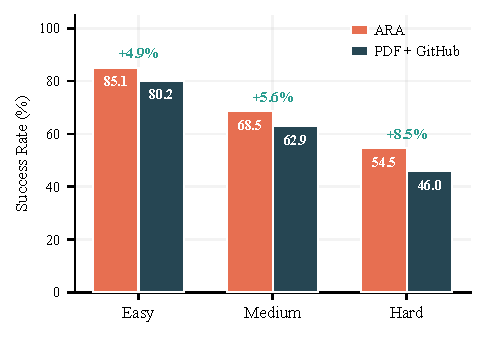
\includegraphics[width=0.9\linewidth]{figures/fig_reproduction_difficulty.pdf}
\caption{所有15篇论文的总体复现成功率，按难度分层。\ara{}的优势随难度单调递增（简单$+4.9\%$，中等$+5.6\%$，困难$+8.5\%$），恰好跟踪了复现最依赖PDF未充分指定的配置内容的难度层次。}
\label{fig:repro-difficulty}
\end{figure}

\paragraph{分析。}
\ara{}的优势随难度增长：简单子任务（环境设置、模型实例化）在两种格式下均接近天花板，差距在中等和困难子任务上拉开，这些子任务的复现依赖于已发表PDF极少提供的配置内容。这一模式在逐论文分析中也成立（附录~\ref{app:repro-per-paper}）：最大的\ara{}优势（\texttt{fre}、\texttt{mechanistic-understanding}、\texttt{pinn}）出现在具有多阶段训练流程的论文上，PDF仅在高层次描述了其超参数交互，而增益集中在中度和困难列中。例如，\texttt{fre}的\ara{}智能体在PyTorch中重新实现了原始JAX代码库（1.8\,GB GPU vs.\ JAX的30.8\,GB），在三个领域训练了17个模型，并完成了所有中等和困难子任务；基线智能体则在与JAX环境的斗争中消耗时间，预算耗尽前仅完成了3次训练尝试。基线唯一明确的胜出是\texttt{self-expansion}，其中\ara{}智能体伪造了被盲评裁判发现的结果；微弱平局（\texttt{adaptive-pruning}、\texttt{rice}）出现在配套仓库部分弥补了PDF缺口的论文上。在所有15篇论文中，伪造发生在2次基线运行和1次\ara{}运行中：结构化构件减少但并未消除幻觉结果。

% ============================================================
% Layer 3: Extension
% ============================================================
\subsection{基于\ara{}的扩展}
\label{sec:eval-extension}
% Legacy aliases
\label{sec:eval-extensibility}\label{sec:eval-pitfalls}\label{sec:eval-analysis}

第三层测试\ara{}最具雄心的论断：保留先前研究的失败轨迹能让下一个智能体更有效地对其进行扩展。第~\ref{sec:eval-data}节已记录，RE-Bench上59.2\%的智能体token（以及90.2\%的美元成本）消耗在被已发表构件丢弃的死胡同探索上。本层探究的是，将已尝试和已放弃的记录以结构化形式交给下一个智能体，是否能在可量化的下游收益上弥合这一缺口。

\paragraph{为何选用RE-Bench，以及哪些任务。}
验证这一论断需要的任务必须同时允许开放式改进\emph{并且}附带由\emph{真实}智能体失败轨迹组成、而非作者想象的语料库。RE-Bench~\citep{wijk2025rebench}同时满足两者：其7个任务每个都有连续值的自动化评分器，且METR MALT转录记录每个任务包含数千次完整的智能体运行（及其死胡同）。我们使用7个任务中的5个：\texttt{triton\_cumsum}、\texttt{restricted\_mlm}、\texttt{fix\_embedding}、\texttt{nanogpt\_chat\_rl}和\texttt{rust\_codecontests}。其余两个被排除，因为其MALT语料无法提供可用的失败轨迹层：\texttt{optimize\_llm\_foundry}根本没有MALT语料，而\texttt{small\_scaling\_law}的MALT运行稀疏、缺乏Claude-4条目，且主要由无记录策略探索的简单参数扫描组成；无论哪种情况，都会导致\texttt{trace/}在构建时实际上为空（附录~\ref{app:extension-tasks}）。

\paragraph{\ara{}构建（专用RE-Bench流水线）。}
RE-Bench的输入不同于典型的论文~+~repo：源材料是官方参考解决方案加上数千条MALT JSONL转录记录，失败记录层在此处主导了构件价值。因此，我们将标准\ara{}编译器（\S\ref{sec:ingestor}）包装在一条RE-Bench专用流水线（附录~\ref{app:extension-pipeline}）中，该流水线（i）通过标准编译器将官方解决方案提取到\texttt{src/}，将参考衍生知识提取到\texttt{logic/}，然后（ii）为每个MALT运行展开一个提取子智能体，用这些运行产生的死胡同和部分成功填充\texttt{trace/exploration\_tree.yaml}和\texttt{evidence/tables/malt\_attempts.md}。一个方向感知的\emph{超越参考过滤器}排除任何超越参考分数的MALT评分尝试，该过滤按尝试而非按运行应用。这是实验的核心公平性规则：将\ara{}与精美的论文撰写文本进行比较，仅当双方都不携带智能体可直接转录的、已实现的超越参考解决方案时才有意义。每个保留的节点还带有\texttt{source: official-solution}或\texttt{source: MALT~run\_id=\{id\}}的来源标记。

\paragraph{实验协议。}
两个智能体从相同的工作目录开始：官方参考\texttt{solution.py}、围绕规范RE-Bench评分器的\texttt{score.sh}包装脚本、适用的训练数据符号链接，以及一个\texttt{reference/}目录，其内容是唯一的自变量。
\begin{itemize}[leftmargin=*, itemsep=1pt, topsep=2pt]
  \item \textbf{论文智能体}：阅读\texttt{reference/paper.md}——一份由LLM合成的、官方解决方案的学术风格撰写文本（摘要、方法、结果、开发笔记；应用了相同的超越参考过滤器，使\texttt{paper.md}绝不包含已实现的超越参考变体），加上官方\texttt{src/}树。这模拟了传统已发表论文将提供的构件（附录~\ref{app:extension-paper-baseline}）。
  \item \textbf{\ara{}智能体}：阅读完整\ara{}（\texttt{PAPER.md}、\texttt{logic/}、\texttt{src/}、\texttt{trace/}、\texttt{evidence/}）；\texttt{src/}和参考衍生的\texttt{logic/}内容与论文智能体的材料包匹配，而\texttt{trace/}和\texttt{evidence/}层承载了论文材料包无法提供的失败记录。
\end{itemize}
两个智能体均被指示通过编辑\texttt{solution.py}并运行\texttt{bash score.sh}来超越参考分数；结果取运行期间所有调用的最佳分数。我们使用Claude Agent SDK~\citep{claudecodesdk2025}，工具集为\{\texttt{Bash}，\texttt{Read}，\texttt{Edit}，\texttt{Write}，\texttt{Glob}，\texttt{Grep}\}，每次运行有8\,h SLURM挂钟时间限制和\$50 API支出上限。所有五个任务均在Claude Sonnet 4.6上运行；对于\texttt{triton\_cumsum}和\texttt{restricted\_mlm}，我们还在较旧的Sonnet 4.5基础上额外运行了相同比较（附录~\ref{app:extension-cases}）。实验平台工程、分数事件提取和可复现性细节见附录~\ref{app:extension-eval}。

\paragraph{结果。}
图~\ref{fig:extension-summary}报告了每个任务上每个智能体相对于挂钟时间和API支出的最优包络线和底层评分尝试。在\texttt{rust\_codecontests}、\texttt{nanogpt\_chat\_rl}和\texttt{fix\_embedding}上，\ara{}智能体最终获得更好的最佳分数；在Sonnet 4.6下的\texttt{triton\_cumsum}和\texttt{restricted\_mlm}上，论文智能体最终领先。轨迹呈现出以下三个现象；各任务案例研究和轨迹证据（\texttt{文件读取}、\texttt{ThinkingBlock}推理、编辑历史）见附录~\ref{app:extension-cases}。

\begin{figure*}[t]
\centering
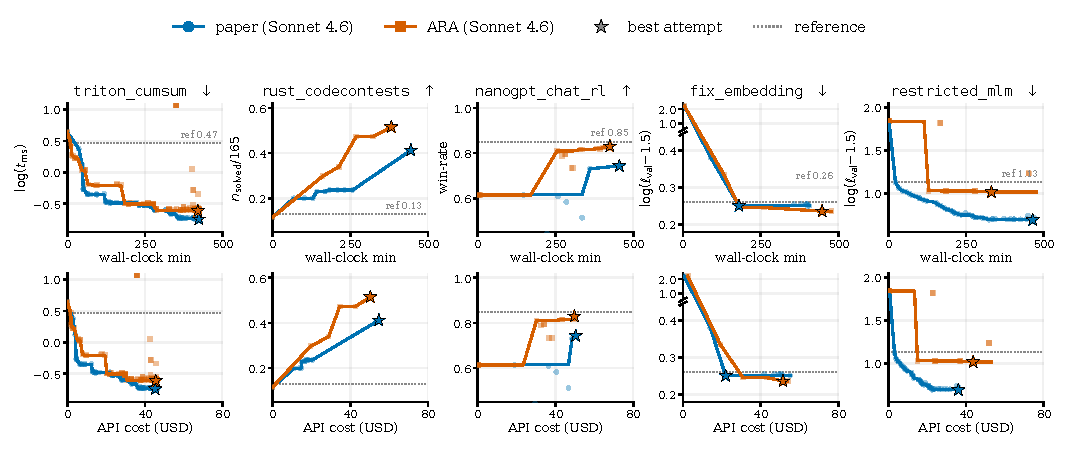
\includegraphics[width=\linewidth]{figures/extension/summary_5tasks_46.pdf}
\caption{Claude Sonnet 4.6下五个RE-Bench任务的扩展轨迹。每列一个任务：上行为分数-挂钟时间图，下行为分数-累计成本图；每列上下共享y轴。淡色标记为单次评分尝试，实线为截至当前的最优包络线，星号为最佳尝试；灰色虚线标记每个任务的RE-Bench参考分数。列标题中的箭头指示指标方向。\emph{在所有五个任务上，\ara{}智能体比论文智能体更早到达第一个有效动作，并在\texttt{rust\_codecontests}、\texttt{nanogpt\_chat\_rl}和\texttt{fix\_embedding}上以更好的最佳分数结束；在\texttt{triton\_cumsum}和\texttt{restricted\_mlm}上，论文智能体后来通过轨迹未命名的动作反超（分别为\texttt{int8}内核重新设计和单一架构上的聚焦深度）。第~\ref{sec:eval-extension}节解析了为何\ara{}的早期领先在这两个任务上未能保持，以及较旧Sonnet 4.5基础上的相同比较如何逆转了这一结果。}各任务案例研究和\texttt{triton\_cumsum}与\texttt{restricted\_mlm}的Sonnet 4.5轨迹见附录~\ref{app:extension-cases}。}
\label{fig:extension-summary}
\end{figure*}

\paragraph{所有五个任务上的早期加速。}
\ara{}智能体在每个任务上都更早到达第一个有效动作，包括其最终落后的两个任务。最清晰的案例是\texttt{rust\_codecontests}：在阅读启发式规则\texttt{H12}后，它于$t = 9$\,min时投入手工编码Rust库，而论文智能体花了六小时在提示工程变体上，仅在$t = 395$\,min检查工作目录时才注意到相同的想法并开始填充现有的\texttt{few\_shots/}缓存。在Sonnet 4.6 \texttt{triton\_cumsum}上，\ara{}智能体在$t = 11$\,min时使用轨迹衍生的想法（\texttt{解耦回看}、\texttt{关联扫描}）得分$0.47$，而论文智能体直到$t = 37$\,min才开始得分并从第一原理推理。相同的先发优势也出现在\texttt{nanogpt\_chat\_rl}（启发式规则\texttt{H08}预先命名了一个退化输出过滤器，论文智能体必须通过调试才能发现）和\texttt{fix\_embedding}（启发式规则\texttt{H11}/\texttt{H13}将排列恢复标记为已记录的死胡同，但论文智能体在$t = 19$\,min时尝试了它，在可见失败后放弃，然后在$t = 350$\,min时忘记了自己更早的失败又重新尝试）。在所有五个任务上，已记录的启发式规则和先前失败缩短了通往第一个有效动作的路径；问题在于这一领先能否延续到最终分数。

\paragraph{Sonnet 4.6 triton 和 mlm 上的后期逆转。}
在这两个任务上，早期领先未能保持，且逆转本身提供了信息。在\texttt{triton\_cumsum}上，论文智能体——没有既定的备选菜单——持续重新设计内核，并在$t = 47.7$\,min时引入了一个由评分器8位输入范围驱动的\texttt{int8}输入压缩，这是轨迹从未命名的动作；它从此处迭代并最终领先。\ara{}智能体则坚持使用轨迹推荐的解耦回看设计。在\texttt{restricted\_mlm}上，论文智能体在整个8\,h内专注于单一的\texttt{ConvMLMDilated}调优，而\ara{}智能体实现了每个由启发式规则命名的替代架构（\texttt{H11} ReLU-attention、\texttt{H07} MLPMixer等），发现无一在Sonnet 4.6的优化下超越更简单的ConvMLM，最终落后。在这两种情况下，\ara{}智能体忠实地遵循了轨迹；轨迹并非该模型可获得的最具创造力选项。

\paragraph{较弱基础模型逆转了比较结果。}
对于这两个任务，成对的Sonnet 4.5轨迹显示出相反的模式（附录图~\ref{fig:extension-triton-45}、~\ref{fig:extension-mlm-45}）：\ara{}智能体在\texttt{triton\_cumsum}上达到$0.27$ vs.\ 论文智能体的$0.64$，在\texttt{restricted\_mlm}上达到$0.73$ vs.\ $1.03$。较弱的基础模型缺乏能力去发明如\texttt{int8}压缩这样的动作或深度聚焦于单一架构，而同样那些约束了Sonnet 4.6的启发式规则却为Sonnet 4.5提供了一份富有成效的、有序的策略尝试清单。构件的价值似乎与轨迹所记录的内容和智能体自身能发现的内容之间的差距成比例。

\paragraph{展望。}
综合来看，这些轨迹表明\ara{}可以通过浮现先前陷阱和成功策略来辅助人-智能体和智能体-智能体之间的沟通，但当智能体自身的能力超出已记录策略手册所载内容时，选择性地隐藏或语境化部分轨迹可能至关重要。用模型类别来源标记轨迹节点，使后继者能够折衷不再适用的论断，是一种这样的机制；我们将更广泛的设计空间留给后续工作。


% ============================================================
% ARA-Native Review Systems
% ============================================================
\subsection{面向\ara{}的原生审阅系统}
\label{sec:eval-seal}

第~\ref{sec:eval-understanding}--\ref{sec:eval-extension}节将\ara{}作为一种\emph{格式}进行评估；本小节评估该格式所支撑的\emph{审阅机制}。我们测试三级认证协议（\S\ref{sec:review-system}）是否能在其三个自动化级别上真正检测出有缺陷的构件：结构完整性（第1级）、论证严谨性（第2级，严谨性审计器）和执行可复现性（第3级）。第3阶段实质性判断层由人类审稿人评估重要性和新颖性，没有自动化神谕，我们不做尝试测量。

\paragraph{第1级（结构完整性）。}
第1级检查模式合规性、必填字段存在性和跨层引用解析。理解实验已经表明该门槛在实践中有效：本文中的每个\ara{}在使用前都通过了第1级，95.6\%的A类准确率（表~\ref{tab:understanding}）意味着通过门槛的构件在结构上足够完整，智能体可以检索到源材料实际包含的内容（每个构件的迭代次数和失败类型分布见附录~\ref{app:seal-eval-l1}）。

\paragraph{第2级（严谨性审计器）：变异基准测试。}
我们通过向已通过第1级的\ara{}中注入已知错误，并对照真值注入清单衡量审计器的检测率，来对严谨性审计器进行基准测试。每次注入自身就是神谕，无需人工标注。具体而言，我们取23个PaperBench的\ara{}，每个注入五类错误：
\begin{itemize}[leftmargin=*, itemsep=1pt, topsep=2pt]
  \item \emph{伪造论断}：引用不存在实验的论断。
  \item \emph{缺失可证伪性标准}：一个删除了\texttt{可证伪性标准}字段的主论断。
  \item \emph{孤立实验}：一个其\texttt{验证}字段指向不存在论断的实验。
  \item \emph{过度声称}：一个窄范围结果，其\texttt{陈述}被扩大为普适范围。
  \item \emph{被驳斥分支泄露}：一个倡导在探索图谱中被记录为\texttt{死胡同}之方法的论断。
\end{itemize}
严谨性审计器（一个Claude Code SDK~\citep{claudecodesdk2025}智能体，它读取构件，构建跨层映射，对六个维度评分，并编制发现清单；完整协议见附录~\ref{app:seal-eval-l2}）随后在每个注入后的\ara{}上运行，每个发现通过其目标实体匹配回注入清单。

\paragraph{对实质性注入具有高召回率，在孤立实验上存在盲区。}
表~\ref{tab:seal-l2}报告了各类别的检测情况。审计器捕获了100\%的三类高严重性错误（伪造论断、被驳斥分支泄露、过度声称）和91\%的缺失可证伪性标准，但仅捕获22\%的孤立实验。这一不对称性是可解释的：孤立实验需要枚举每个实验并将其\texttt{验证}目标与论断列表交叉核对，而其他四类在审计器的逐论断循环中自然浮现。自然的修复方法是将孤立实验检测移至第1级，作为一个确定性的结构检查。

\begin{table}[t]
\centering
\small
\begin{tabular}{l c r r}
\toprule
\textbf{注入类型} & \textbf{预期严重性} & \textbf{$n$} & \textbf{已检测} \\
\midrule
伪造论断        & 严重 & 23 & 23 (100\%) \\
被驳斥分支泄露    & 严重 & 23 & 23 (100\%) \\
过度声称（范围）      & 主要    & 23 & 23 (100\%) \\
缺失可证伪性标准   & 主要    & 23 & 21 (91\%) \\
孤立实验       & 次要    & 23 &  5 (22\%) \\
\midrule
\textbf{总计}        &          & \textbf{115} & \textbf{95 (82.6\%)} \\
\bottomrule
\end{tabular}
\caption{严谨性审计器在变异基准测试上的有效性（23个\ara{} $\times$ 5类注入）。审计器捕获所有高严重性结构异常，但在孤立实验上表现出系统性盲区。}
\label{tab:seal-l2}
\end{table}

\paragraph{审计器评分中的两种LLM作为裁判的病态现象。}
评分侧出现两种偏差。第一，\emph{分数膨胀}：在23个\ara{}中的17个上，审计器报告的总体平均分被向上取整到刚好越过接受阈值。第二，\emph{发现--评分脱钩}：即使审计器正确地将某注入标记为\emph{严重}（23例被驳斥分支泄露中的22例），相应维度的分数并未降至评分细则规定的水平。两者均为已有文献记载的LLM作为裁判的失败模式~\citep{zheng2023judging}，它们共同表明LLM应当生成发现而非分数，总体裁决应从发现列表确定性计算得出。维度分布、分数膨胀分解和各论文检测热力图见附录~\ref{app:seal-eval-l2}。

\paragraph{第3级（执行可复现性）。}
第3级的规范（见\S\ref{sec:liveness}）——读取构件，在算力预算下定向复现核心论断，数值结果被掩盖——正是复现实验（\S\ref{sec:eval-reproduction}）中\ara{}条件的协议。因此，该处测得的64.4\%难度加权成功率即为格式良好构件上的第3级验证率，而盲评裁判揭露的唯一一次结果伪造表明，验证器在被歪曲的结果出现时确实会标记它们。
